\chapter{Results and Discussion}

The data and discussion of results below come in a combination of data gathered using the OONI probe in Ireland and Iraq, as well as published OONI data from the OONI Measurement Aggregation Toolkit (MAT).

\section{Summary of Test Results}

The tested results yielded expected results - Ireland primarily blocked pirated and illegal content, while Iraq blocked a wider range of content.

[expanded stuff will go here]

\subsection{Website Accessibility Results}

The results below are an average of the number of websites blocked each day over the testing period of 15 days.

\begin{table}[H]
\centering
\caption{Summary of Blocked vs. Unblocked Websites by Country}
\begin{tabular}{lcc}
\toprule
\textbf{Country} & \textbf{Unblocked} & \textbf{Blocked} \\
\midrule
Ireland & X & Y \\
Iraq    & A & B \\
\bottomrule
\end{tabular}
\label{tab:blocked_summary}
\end{table}

The table below shows the frequency of block methods found in Iraq.

\begin{table}[H]
\centering
\caption{Distribution of Blocking Methods Detected in Iraq}
\begin{tabular}{lc}
\toprule
\textbf{Blocking Method} & \textbf{Frequency} \\
\midrule
TCP/IP          & N1 \\
DNS & N2 \\
HTTP & N3 \\
\bottomrule
\end{tabular}
\label{tab:iraq_blocking_methods}
\end{table}

The table below shows the frequency of block methods found in Ireland.

\begin{table}[H]
\centering
\caption{Distribution of Blocking Methods Detected in Ireland}
\begin{tabular}{lc}
\toprule
\textbf{Blocking Method} & \textbf{Frequency} \\
\midrule
TCP/IP          & N1 \\
DNS & N2 \\
HTTP & N3 \\
Unidentified & N3 \\
\bottomrule
\end{tabular}
\label{tab:ireland_blocking_methods}
\end{table}

The table below shows the number of websites blocked in each category in both countries.

\begin{table}[H]
\centering
\caption{Blocked Websites by Category and Country}
\begin{tabular}{lcc}
\toprule
\textbf{Category} & \textbf{Ireland} & \textbf{Iraq} \\
\midrule
Uncategorized                       & -- & -- \\
Piracy / Streaming / File Sharing   & -- & -- \\
News / Media                        & -- & -- \\
Adult Content                       & -- & -- \\
Creative / Educational / Misc       & -- & -- \\
General / National Services         & -- & -- \\
Streaming / Social Media            & -- & -- \\
Religious                           & -- & -- \\
VoIP / Communication                & -- & -- \\
Gambling                            & -- & -- \\
Email/Privacy Tools                 & -- & -- \\
Adult / Alcohol                     & -- & -- \\
LGBTQ+                              & -- & -- \\
AI / Technology                     & -- & -- \\
\bottomrule
\end{tabular}
\label{tab:category_block}
\end{table}

\subsection{Circumvention Test Results}

Ireland and Iraq yielded similar 

\subsubsection{Ireland}

Ireland likely does not block Tor on any of its ASNs, as it is largely accessible outside of 2 anomalies.

\textbf{March 18, 2025} - Magnet Networks Limited (AS34245) - Tor Test (1 anomaly out of 78 measurements)
%https://explorer.ooni.org/m/20250318181530.182975_IE_tor_8b558463294b2881

\textbf{March 31, 2025} - Liberty Global B.V. (AS6830) - Tor Test (1 anomaly out of 191 measurements)
%https://explorer.ooni.org/m/20250331102020.562562_IE_tor_913ee551111fe0a9

Outside of these two anomalies, there is no evidence that Tor is being blocked in Ireland.

Psiphon on the other hand yielded different results. While Psiphon was largely able to be accessed on most ASNs, there were a few where access is likely blocked. 

\begin{table}[H]
\centering
\caption{ASN's with Evidence of Psiphon being Blocked in Ireland}
\begin{tabular}{lccc}
\toprule
\textbf{ASN} & \textbf{Anomaly} & \textbf{Total Measurement Count} & \textbf{Percentage} \\
\midrule
AS1213    & 33 & 35  & 94\% \\
AS6830    & 16 & 215 & 7.4\% \\
AS8075    & 1  & 1   & 100\% \\
AS13280   & 8  & 12  & 66\% \\
AS15751   & 1  & 9   & 11\% \\
\bottomrule
\end{tabular}
\label{tab:category_block}
\end{table}

\subsubsection{Iraq}

Similar to Ireland, Iraq largely does not block access to Tor outside of a few outliers.

\textbf{March 20, 2025} - Super Cell Network for Internet Services LTD (AS209193) - Tor Test (1 anomaly out of 92 measurements)
%https://explorer.ooni.org/m/20250320220102.873661_IQ_tor_3796e6aaa913670d

\textbf{March 30, 2025} - Hulum Almustakbal Company for Communication Engineering and Services Ltd (AS203214) - Tor Test (2 anomalies out of 160 measurements)
%https://explorer.ooni.org/m/20250330191838.341920_IQ_tor_f0e7ccd345c39d7f

\textbf{March 30, 2025} - Valin Company for General Trading and Communications LTD (AS205254) - Tor Test (1 anomaly out of 17 measurements)
%https://explorer.ooni.org/m/20250330111106.914884_IQ_tor_f45745fcedc21407

Outside of these anomalies, there is no significant evidence that Tor is being blocked in Iraq.

There is also little evidence of Psiphon being blocked in Iraq at a significant scale. Aside of a few outliers, Psiphon only seemed to be blocked on one ASN. 

\begin{table}[H]
\centering
\caption{ASN's with Evidence of Psiphon being Blocked in Iraq}
\begin{tabular}{lccc}
\toprule
\textbf{ASN} & \textbf{Anomaly} & \textbf{Total Measurement Count} & \textbf{Percentage} \\
\midrule
AS203214  & 127 & 165  & 77\% \\
AS51684   & 4   & 23   & 17\% \\
AS199739  & 1   & 352  & 0.2\% \\
AS205254  & 1   & 30   & 3.3\% \\
AS208324  & 1   & 3    & 33\% \\
\bottomrule
\end{tabular}
\label{tab:category_block}
\end{table}

Based on this data, Psiphon is widely accessible in Iraq outside of AS203214.

\subsection{Instant Messaging Test Results}

The results of the Instant Messaging tests were very similar in Ireland and Iraq. Both tests showed no signs of interference or blocking of Facebook Messenger, Telegram, Whatsapp, or Signal. However, looking outside of the tested ASNs reveals a significant difference between the two countries. The tested data in Ireand is consistent with public OONI data, and shows no blocking of instant messaging platforms. The Iraq data is also consistent with tests run on the same ASN, but in Iraq there are other ASNs that show signs of blocking.

\subsubsection{Ireland}

In the past 30-day period, there were only 2 anomalies found that shows any kind of instant messaging blocking:

\textbf{March 24, 2025} - Packethub S.A. (AS136787) - Facebook Messenger Test (1 anomaly out of 3 measurements)
%https://explorer.ooni.org/m/20250324111124.418686_IE_facebookmessenger_fbdc8895400acaba

\textbf{March 24, 2025} - HEAnetCLG (AS1213) - Signal Test (1 anomaly out of 37 measurements)
%https://explorer.ooni.org/m/20250324164458.153631_IE_signal_667f7ad13e55043a

Outside of these anomalies, there was no evidence of instant messaging blocking.

\subsubsection{Iraq}

Iraq had significant evidence of instant messaging platforms being blocked in certain ASNs. The table below shows each ASN, and the percentage of tests where there was an anomaly found.

\begin{table}[H]
\centering
\caption{ASN's with Evidence of Instant Message Platform Blocking in Iraq}
\begin{tabular}{lcccc}
\toprule
\textbf{ASN} & \textbf{Facebook} & \textbf{Telegram} & \textbf{WhatsApp} & \textbf{Signal} \\
\midrule
AS203214  & 27\%  & 7.8\% & 25\%  & 44\% \\
AS205254  & 26\%  & 3.8\% & 7.6\% & 7.6\% \\
AS199739  & 1\%   & 0.5\% & 0.2\% & 0.8\% \\
AS13335   & 47\%  & 0\%   & 0\%   & 0\% \\
AS50710   & 33\%  & 0\%   & 0\%   & 0\% \\
AS206206  & 60\%  & 0\%   & 0\%   & 0\% \\
AS212330  & 100\% & 0\%   & 0\%   & 0\% \\
AS210022  & 0\%   & 0\%   & 0\%   & 82\% \\
AS51020   & 0\%   & 0\%   & 0\%   & 32\% \\
AS202651  & 0\%   & 0\%   & 0\%   & 23\% \\
AS59588   & 0\%   & 0\%   & 1.9\% & 1.9\% \\
AS209193  & 0\%   & 0\%   & 0.7\% & 0\% \\
\bottomrule
\end{tabular}
\label{tab:category_block}
\end{table}

Instant Messaging platforms are essentially widely available in Iraq, but there are some areas where blocking does occur.

\subsection{Middlebox Test Results}

The results of the Middlebox Test were the same for both countries. Both the HTTP Header Field Manipulation and HTTP Invalid Request Line tests resulted in no Middleboxes being detected in either country. However, while there was no evidence of Middleboxes being found using the providers tested, it is possible that other providers in both countries have Middleboxes present in the network.

Using publicly available OONI data for Ireland and Iraq, it was found that there were cases of Middleboxes being detected in both countries over the past 30 days (March 6, 2025 - April 6, 2025). 

\subsubsection{Ireland}

There is very little evidence of Middleboxes being present in Ireland. Over the past 30-day period, there are only two anomalies present. Both of these anomalies are from the HTTP Invalid Request Line test. 

\textbf{March 25, 2025} - Meteor Mobile Communications Ireland (AS15751) (1 anomaly out of 9 measurements)
%https://explorer.ooni.org/m/20250325122211.663367_IE_httpinvalidrequestline_c713442d98eebb5c

\textbf{April 1, 2025} - Vodafone Ireland Limited (AS15502) (1 anomaly out of 79 measurements)
%https://explorer.ooni.org/m/20250401215651.365763_IE_httpinvalidrequestline_51f20fe7e9d31698

These results are likely outliers, as there are very little Middlebox tests for Meteor Mobile Communications Ireland in this time span and no other anomalies for Vodafone Ireland Limited.

\subsubsection{Iraq}

There is considerably more evidence of Middleboxes being present in Iraq. Over the past 30 day period, there were 125 anomalies in the HTTP Invalid request line Test and 19 anomalies in the HTTP Header Field Manipulation Test.

The table below lists the ASNs that were suspected to have Middleboxes present using the HTTP Invalid Request Line test. It then shows the number of anomalies, the total measurement count, and what percentage of the total count were anomalies. Note that any ASN that had less than 0.5\% anomalies was ignored.

\begin{table}[H]
\centering
\caption{ASN's with Evidence of Middleboxes (HTTP Invalid Request Line Test) in Iraq}
\begin{tabular}{lccc}
\toprule
\textbf{ASN} & \textbf{Anomaly} & \textbf{Total Measurement Count} & \textbf{Percentage} \\
\midrule
AS13335   & 8 & 10 & 80\% \\
AS59588   & 13 & 53 & 24.5\% \\
AS48492   & 2 & 4 & 50\% \\
AS50710   & 1 & 1 & 100\% \\
AS198589  & 68 & 70 & 97\% \\
AS203214  & 32 & 158 & 20.25\% \\
\bottomrule
\end{tabular}
\label{tab:category_block}
\end{table}

\begin{figure}[H]
    \centering
    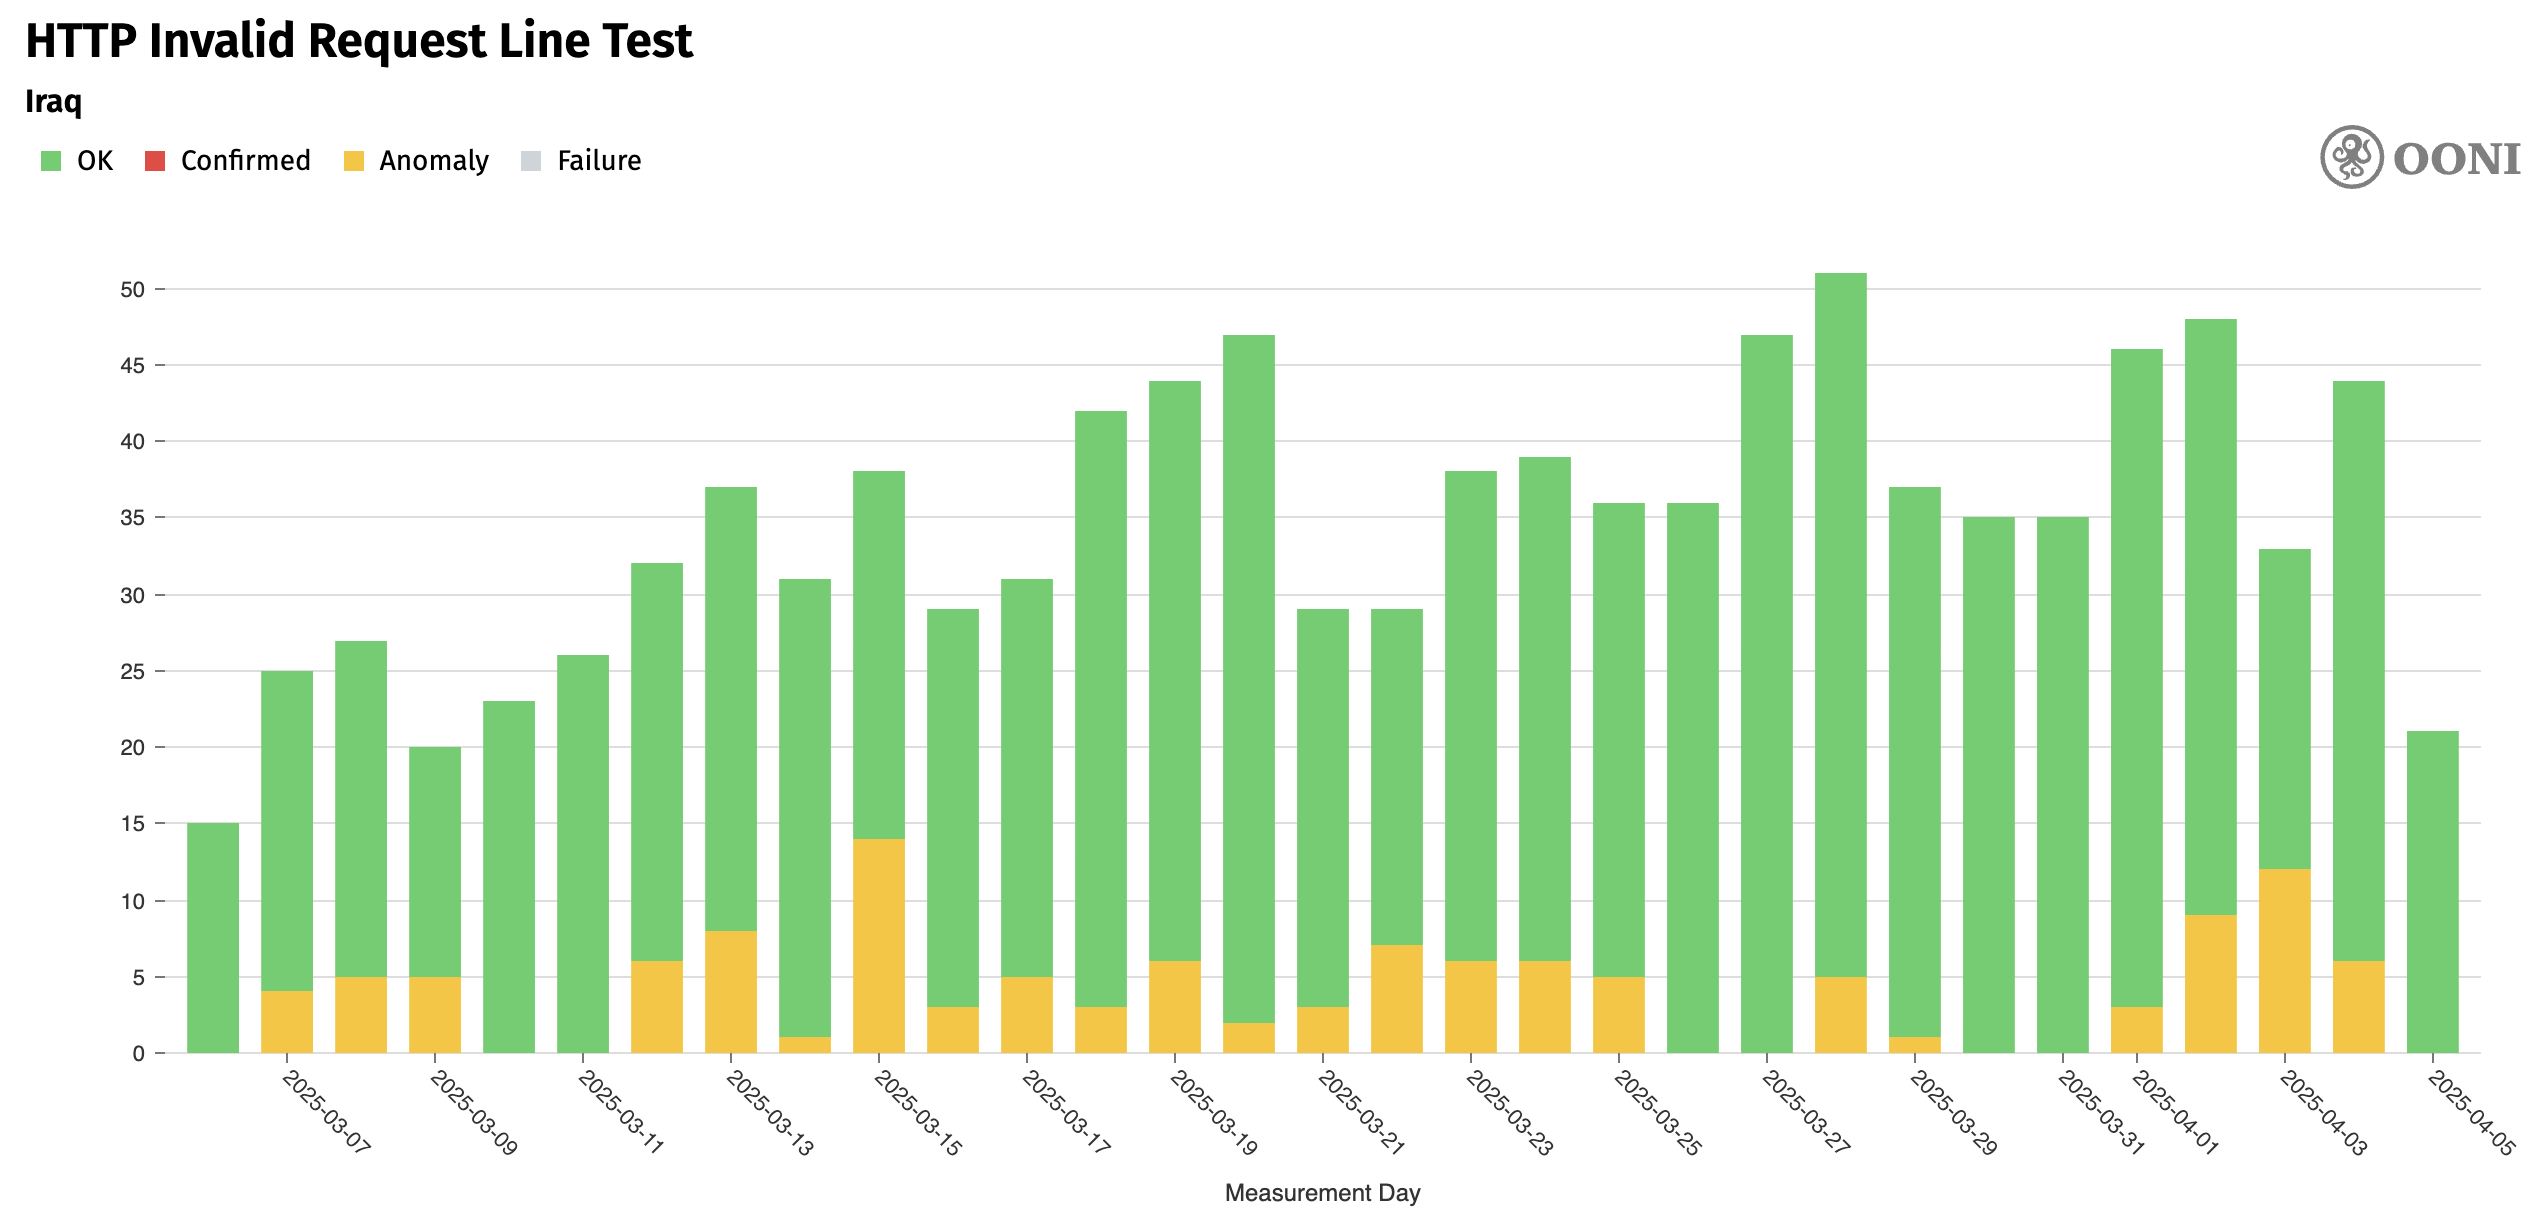
\includegraphics[width=\textwidth]{Griff/TCD SCSS CAPSTONE/Results/IraqMiddleboxHTTPInvalidTest.png}
    \caption{Iraq Middlebox HTTP Invalid Request Line Test: March 6, 2025 -- April 6, 2025}
    \label{fig:iraq-middlebox-invalid-request}
\end{figure}

The table below lists the ASNs that were suspected to have Middleboxes present using the HTTP Header Field Manipulation test. It then shows the number of anomalies, the total measurement count, and what percentage of the total count were anomalies. Note that any ASN that had less than 0.5\% anomalies was ignored.

\begin{table}[H]
\centering
\caption{ASN's with Evidence of Middleboxes (HTTP Header Field Manipulation Test) in Iraq}
\begin{tabular}{lccc}
\toprule
\textbf{ASN} & \textbf{Anomaly} & \textbf{Total Measurement Count} & \textbf{Percentage} \\
\midrule
AS13335   & 8 & 10 & 80\% \\
AS48492   & 2 & 4 & 50\% \\
AS50710   & 1 & 1 & 100\% \\
\bottomrule
\end{tabular}
\label{tab:category_block}
\end{table}

\begin{figure}[H]
    \centering
    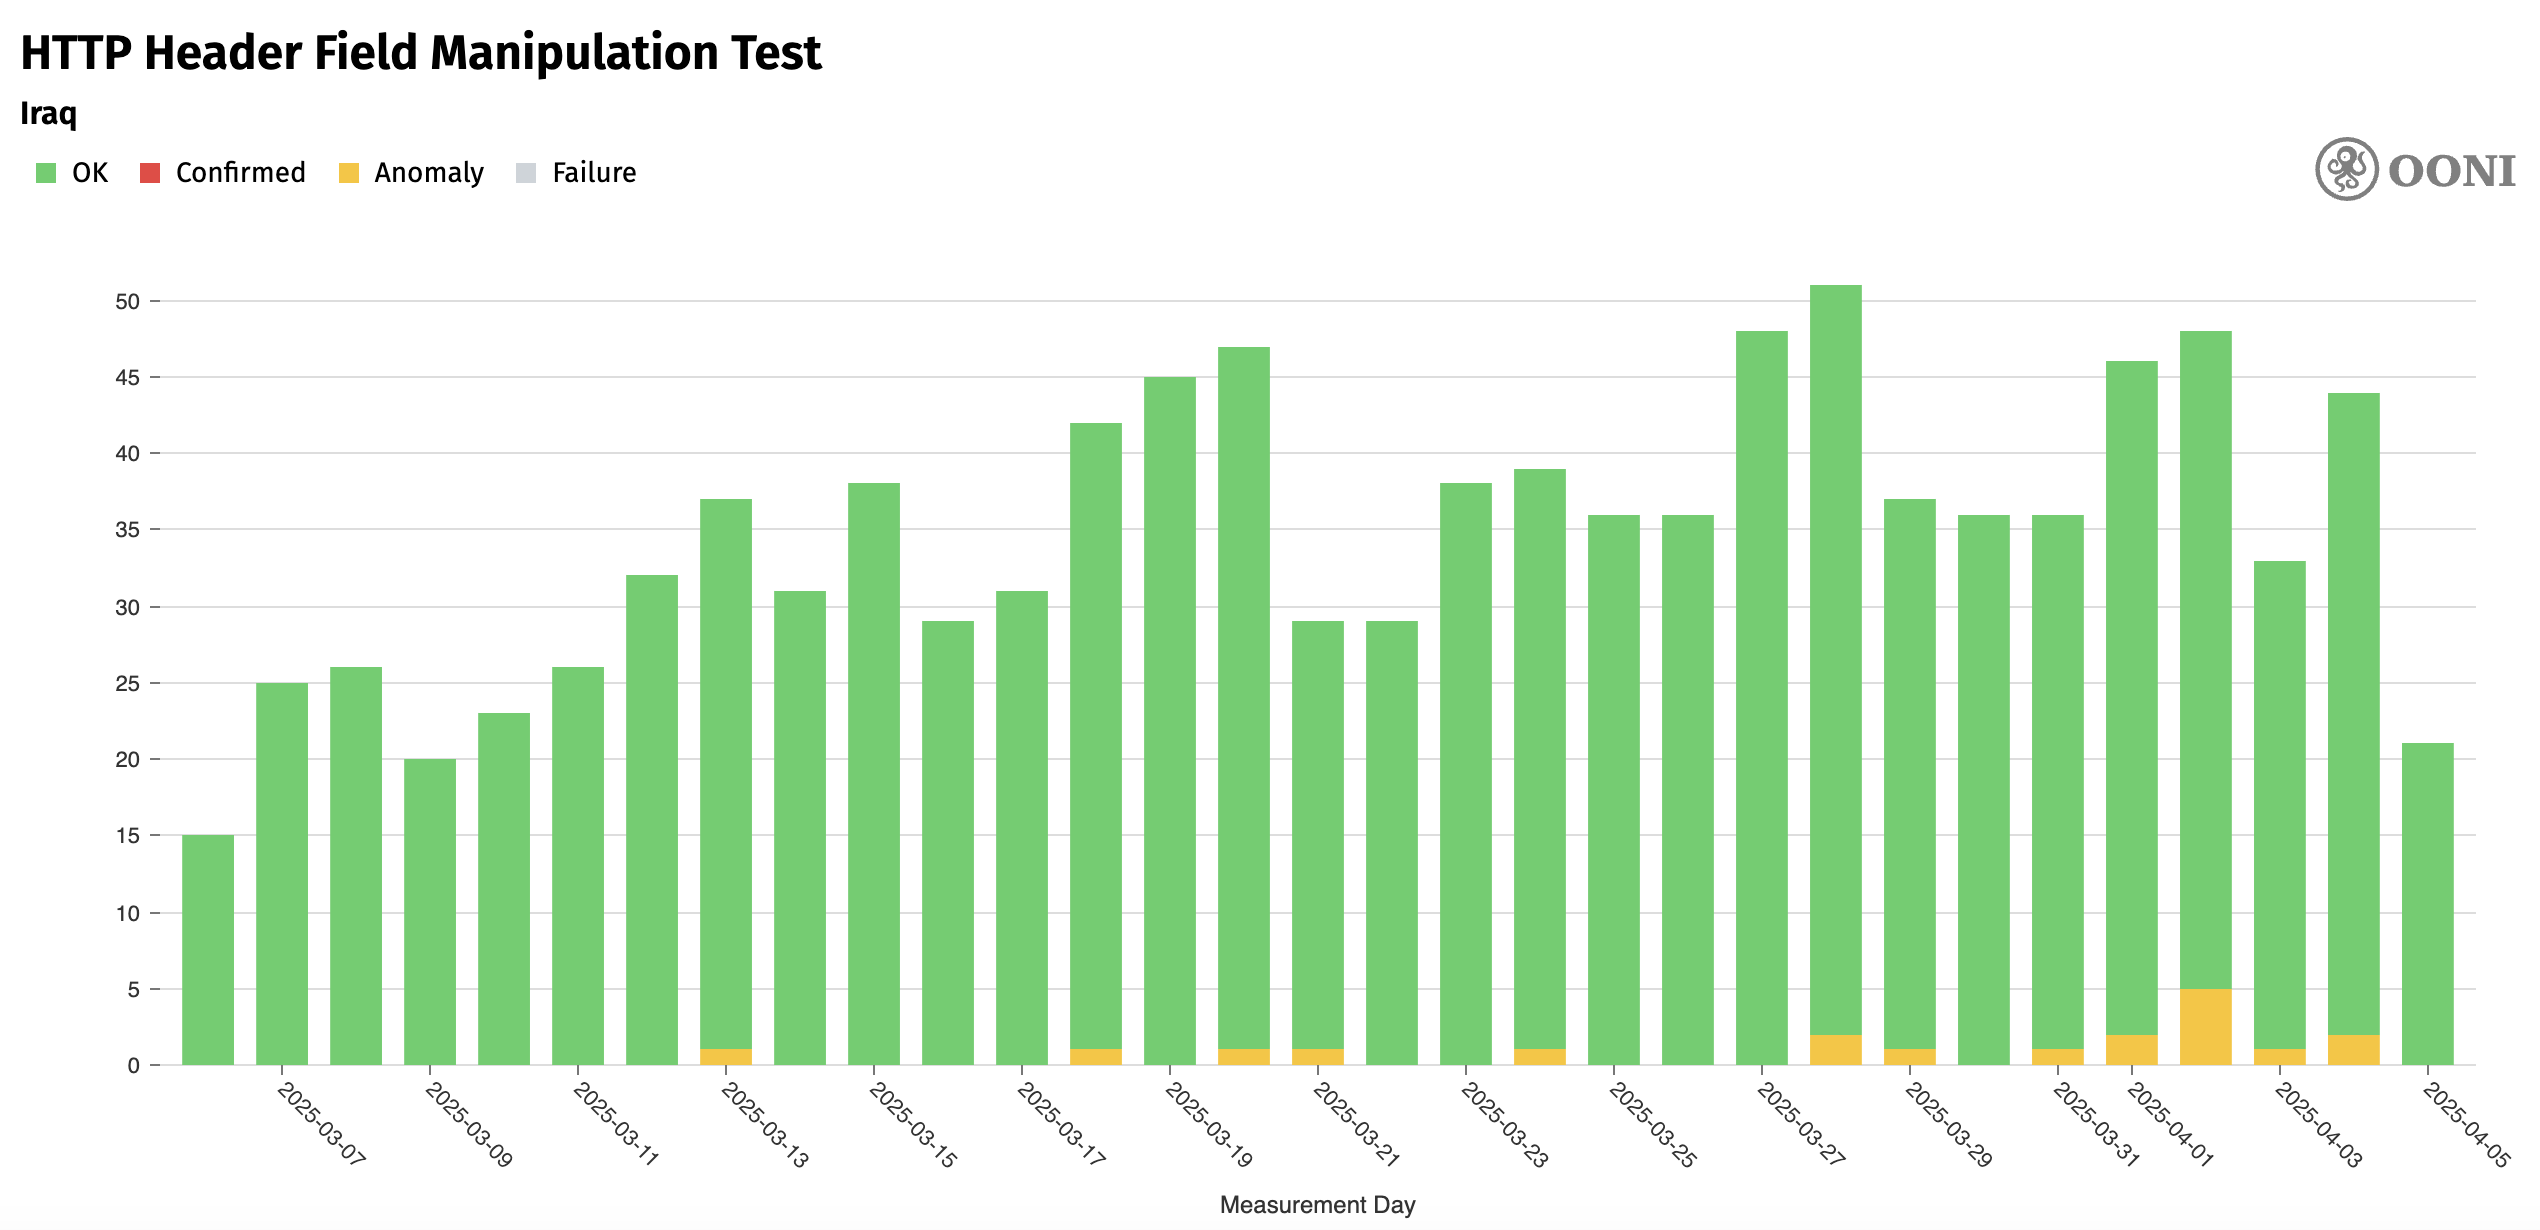
\includegraphics[width=\textwidth]{Griff/TCD SCSS CAPSTONE/Results/IraqMiddleboxHTTPManipulation.png}
    \caption{Iraq Middlebox HTTP Header Field Manipulation Test: March 6, 2025 -- April 6, 2025}
    \label{fig:iraq-middlebox-HTTP-manipulation}
\end{figure}

\textit{Note: All CSV files gathered from the public OONI database can be found on the public GitHub for this work; see Appendix A1.2.}


\section{Comparative Analysis: Ireland v. Iraq}



\subsection{Observed Patterns and Anomalies}



